%%%%%%%%%%%%%%%%%%%%%%%%%%%%%%%%%%%%%%%%%%%%%%%%%%%%%%%%%%%%

\section{Exploring \Wikipedia{} with \WikiTax} 
\label{S:approach}

%%%%%%%%%%%%%%%%%%%%%%%%%%%%%%%%%%%%%%%%%%%%%%%%%%%%%%%%%%%%

\vspace{-27\in}

\paragraph*{\textbf{\Wikipedia's category graph}}

\Wikipedia{} uses several means of organizing its information: plain
links giving rise to an article graph, designated article lists,
portals meant to introduce users to key topics, info-boxes for
semantic (`typed') data, and categories giving rise to a category
graph for the classification of articles. When it comes to taxonomy
mining, the category graph is particularly relevant; the graph is
accessible, for example, through the \MediaWiki{} API, which is the
access path chosen by \WikiTax.

% \footnote{\url{http://www.mediawiki.org/wiki/API:Main_page}}

%%%%%%%%%%%%%%%%%%%%%%%%%%%%%%%%%%%%%%%%%%%%%%%%%%%%%%%%%%%%

\vspace{-27\in}

\paragraph*{\textbf{Graph extraction}}

Initially, \WikiTax{} is pointed to a root category (level 0) for
extraction. Iteratively, subcategories and pages (in fact, page
titles) can be extracted level by level or exhaustively. Exhaustive
extraction may take minutes to hours depending on the root
category. The \Wikipedia{} category graph contains many surprising
edges, which would easily imply inclusion of large, arguably
irrelevant subgraphs. Thus, extraction is controllable.

%%%%%%%%%%%%%%%%%%%%%%%%%%%%%%%%%%%%%%%%%%%%%%%%%%%%%%%%%%%%

\vspace{-27\in}

\paragraph*{\textbf{Graph reduction}}

\WikiTax{} supports reduction of the graph---both during
(level-by-level) extraction and post extraction. Reduction boils down
to the exclusion of nodes, i.e., categories. (In fact, we may also
remove individual edges, given that a category may have multiple
parent categories.)  A category would be removed, if domain knowledge
suggests that the category at hand does not serve the intended kind of
classification, e.g., classification of software languages in our
case. When exclusion is performed during extraction, then the excluded
nodes (edges) are ignored during subsequent extraction steps. When
exclusion is performed post extraction, then nodes (edges) are only
blacklisted, without actually reducing the graph. In this manner,
exclusion decisions can be revisited.

%%%%%%%%%%%%%%%%%%%%%%%%%%%%%%%%%%%%%%%%%%%%%%%%%%%%%%%%%%%%

\begin{figure}[t!]
\begin{center}
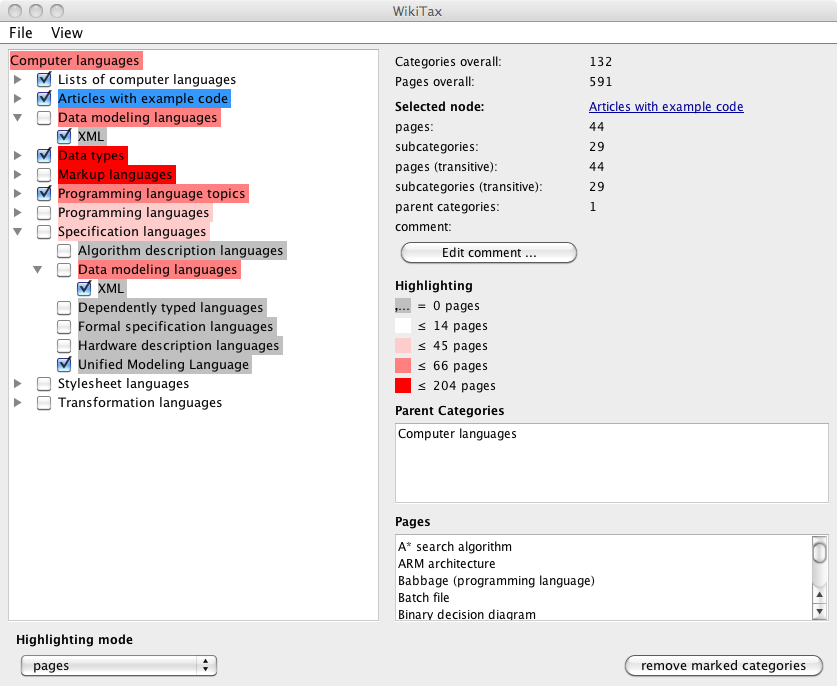
\includegraphics[width=.98\textwidth]{figures/clLevel12.png}
\end{center}
\vspace{-66\in}
\caption{Exploration of level 1 and 2 subcategories of \emph{Computer languages}.}
\label{F:clLevel12}
\vspace{-42\in}
\end{figure}

%%%%%%%%%%%%%%%%%%%%%%%%%%%%%%%%%%%%%%%%%%%%%%%%%%%%%%%%%%%%

\vspace{-27\in}

\paragraph*{\textbf{\WikiTax's visualization}}

\autoref{F:clLevel12} shows the \WikiTax{} exploration view after the
extraction of levels 1 and 2 starting from the category
\WikipediaCategory{Computer languages}. Some edges are marked for
exclusion. (Exclusion would be confirmed with the `removal'
button.)  The marked categories are to be excluded because domain
knowledge suggests that these categories do not serve language
classification in a conceptual manner. Highlighting is
applied to the categories according to the metric of immediate member
pages. In the figure, the category \WikipediaCategory{Articles with
  example code} is selected so that extra data is shown in the panel
on the right, e.g., member pages. All categories and pages are
clickable to navigate to \Wikipedia.

%%%%%%%%%%%%%%%%%%%%%%%%%%%%%%%%%%%%%%%%%%%%%%%%%%%%%%%%%%%%

\begin{figure}[ht]
\centering
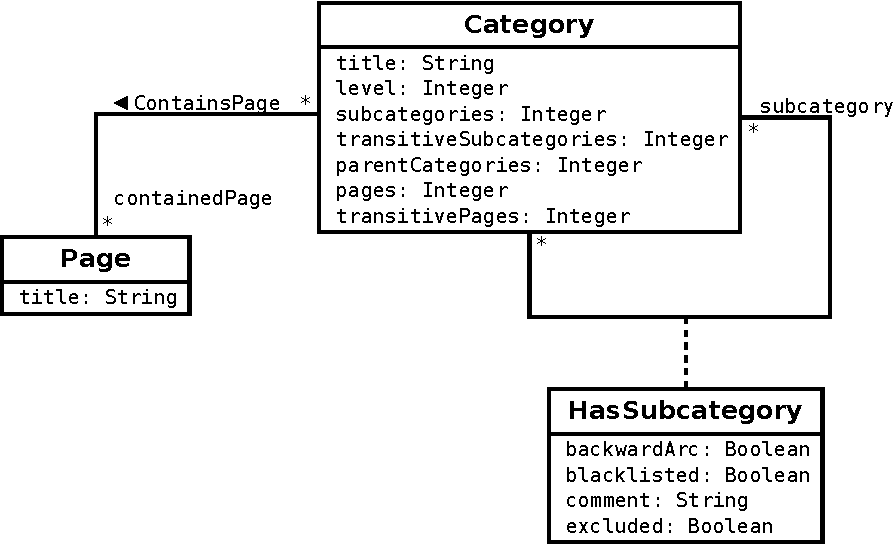
\includegraphics[width=0.75\textwidth]{figures/full_schema.pdf} 
\caption{Metamodel of the \WikiTax{} category graph.}
\label{F:metamodel}
\vspace{-42\in}
\end{figure}

%%%%%%%%%%%%%%%%%%%%%%%%%%%%%%%%%%%%%%%%%%%%%%%%%%%%%%%%%%%%

\vspace{-27\in}

\paragraph*{\textbf{\WikiTax's metamodel}}

\WikiTax{} operates on an enhanced category graph; see the metamodel
in \autoref{F:metamodel}. Thus, each category associates with contained pages and
subcategories. The subcategory associations are attributed to keep
track of metadata as follows:

\vspace{-27\in}

{\small

\begin{description}
\item[\ \ backwardArc] Marker for cyclic edges in the category graph.
\item[\ \ blacklisted] Marker for categories blacklisted past extraction.
\item[\ \ excluded] Marker for categories excluded during reduction.
\item[\ \ comment] Label (`reason for exclusion') to be associated with the edge.
\end{description}

}

\noindent
Categories are associated with measures as follows:

\vspace{-27\in}

{\small

\begin{description}
\item[\ \ level] The level 0, 1, 2, ... of the category in the graph with the root at level 0.
\item[\ \ subcategories] The number of immediate subcategories.
\item[\ \ transitiveSubcategories] The number of all subcategories.
\item[\ \ pages] The number of immediately contained pages.
\item[\ \ transitivePages] The number of all pages in this category.
\end{description}

}

\noindent
The implementation of \WikiTax{} uses the Java-based JGraLab
library\footnote{\url{https://github.com/jgralab}} for the
  representation of (annotated) graphs with JSON as an export format.

%%%%%%%%%%%%%%%%%%%%%%%%%%%%%%%%%%%%%%%%%%%%%%%%%%%%%%%%%%%%

\vspace{-27\in}

\paragraph*{\textbf{Exclusion types}} A methodologically important
aspect of graph reduction is that reasons for category exclusion are
not just simply documented by a comment, but a manageable,
well-defined set of exclusion types is to be developed over time. For
instance, the category \WikipediaCategory{Unified Modeling Language}
could be said to be of an exclusion type `Singleton classifier' to
mean that this category, by design, is primarily concerned with a
single language, i.e., UML in this case; the other members or
subcategories of the category are concerned with UML concepts, tools,
and other related artifacts. \S\ref{S:study} lists several more
exclusion types. The aggregation and use of exclusion types captures
domain knowledge and insight into \Wikipedia's category graph in a
transparent manner.

%%%%%%%%%%%%%%%%%%%%%%%%%%%%%%%%%%%%%%%%%%%%%%%%%%%%%%%%%%%%
